\clearpage

\lehead[]{\normalfont\sffamily\hspace*{-2.00cm}\textcolor{white}{\colorbox{lightblue}{\parbox[c][0.70cm][b]{1.60cm}{
\makebox[1.60cm][r]{\thechapter}\\ \makebox[1.60cm][r]{ÜBUNG}}}}\hspace{0.17cm}\textcolor{lightblue}{\chaptertitle}}
\rohead[]{\textcolor{lightblue}{\chaptertitle}\normalfont\sffamily\hspace*{0.17cm}\textcolor{white}{\colorbox{lightblue}{\parbox[c][0.70cm][b]{1.60cm}{\thechapter\\
ÜBUNG}}}\hspace{-2.00cm}}
%\chead[]{}
\rehead[]{\textcolor{lightblue}{AvHG, Inf, My}}
\lohead[]{\textcolor{lightblue}{AvHG, Inf, My}}

\section{UML-Zustandsdiagramme -- Übungen}

\vspace{1mm}

\begin{minipage}{0.9\textwidth}
\subsection{Aufgabe 1: Windows}
\end{minipage}
\begin{minipage}{0.1\textwidth}
\begin{center}

\includegraphics[width=1.0\textwidth]{./inf/SEKII/11_UML_Zustandsdiagramme/windows.png}
\end{center}
\end{minipage}

Unter dem Betriebssystem Windows lässt sich der Zustand eines Programmfensters
durch Knöpfe verstellen, die sich rechts oben am Fenster befinden (siehe
Abbildung). Beschreibe in einem Zustandsdiagramm, wie man den Zustand eines
Programmfensters verändern kann. Berücksichtige in deinem Zustandsdiagramm auch
die Möglichkeit den Zustand eines Fensters über das Kontextmenü in der
Taskleiste, oder auch durch einfachen Klick auf den entsprechenden Eintrag in
der Taskleiste, zu verändern.

Nimm dabei an, dass das Fenster direkt nach dem Programmstart nur einen Teil des
Bildschirms belegt.



\subsection{Aufgabe 2: Fähre}

Es soll eine Computersimulation für eine Fähre erstellt werden. Zeichne dafür
ein UML-Zustandsdiagramm, das die verschiedenen Zustände der Fähre darstellt:

\begin{quotation}
Die Fähre wartet zehn Minuten am östlichen Ufer
bis alle Personen und Transportmittel an Bord
sind. Dann fährt sie in westlicher Richtung bis zum
anderen Ufer. Am West-Ufer wartet die Fähre
wieder zehn Minuten, bis alle Personen und
Transportmittel aus- beziehungsweise
eingestiegen sind. Anschließend fährt sie in
östlicher Richtung bis sie wieder den Landeplatz
am Ost-Ufer erreicht hat. Dieser Zyklus wiederholt
sich den ganzen Tag lang. Nachts legt die Fähre
am Ost-Ufer an. Dem entsprechend startet sie am
frühen Morgen vom Ost-Ufer aus.
\end{quotation}

\begin{center}
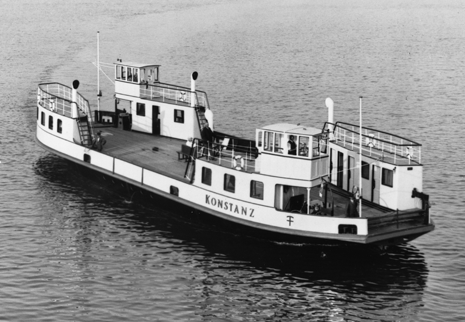
\includegraphics[width=0.4\textwidth]{./inf/SEKII/11_UML_Zustandsdiagramme/faehre.png}
\end{center}
% Anfrage per e-Mail an Uwe.Fiedler@t-online.de am 28.9.13
%
% Antwort am selben Tag:
% Hallo Herr Meyer,
%
% klar - sehr gerne.
%
% Viele Grüße, Uwe Fiedler

\subsection{Aufgabe 3: Seehund}

In einem Computerspiel soll ein Seehund dargestellt werden.
Zeichne dafür ein UML-Zustandsdiagramm, das die
verschiedenen Zustände veranschaulicht, in denen sich der
Seehund des Computerprogramms befinden kann:

\begin{quotation}
Zu Beginn schwimmt der Seehund ziellos im Wasser herum.
Sobald ein Fisch erscheint, verfolgt er diesen. Nachdem er den
Fisch gefangen hat, isst er ihn (längerer Vorgang). Falls dies der
dritte Fisch war, den er gefangen hat, ist er satt und ruht sich auf
einer Sandbank aus. Die Seehund-Simulation ist damit zu Ende.
Andernfalls schwimmt er weiter, um erneut einen Fisch zu
fangen.
\end{quotation}


\subsection{Aufgabe 4: Getränke-Automat}

Schreibe ein Zustandsdiagramm, das die Funktionsweise eines Cola-Automaten
graphisch darstellt:

\begin{quotation}
Eine Dose kostet einen Euro. Man kann jedoch auch andere Münzen in den Automaten
einwerfen. Der Automat gibt gegebenenfalls Wechselgeld zurück. Nach dem Einwurf der
Münzen muss man einen Knopf drücken, damit der Automat weiß, dass die Eingabe der
Münzen abgeschlossen ist. Wenn der Automat leer ist oder wenn der Benutzer zu wenig
Geld eingeworfen hat, wird das Geld wieder zurück gegeben. Andernfalls gibt der
Automat zuerst eine Cola-Dose aus. Anschließend gibt der Automat das Wechselgeld
zurück, falls der eingeworfene Geldbetrag höher als ein Euro war.
\end{quotation}


\subsection{Aufgabe 5: xkcd: My Problem With Phone Alarms}

Interpretiere das folgende \glqq Zustandsdiagramm\grqq :

\begin{center}
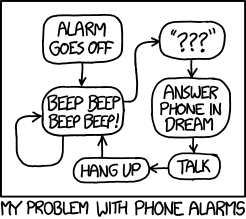
\includegraphics[width=0.5\textwidth]{./inf/SEKII/11_UML_Zustandsdiagramme/phone_alarm.png}
\end{center}
% Creative Commons Attribution-NonCommercial 2.5 License

(Quelle: \url{http://xkcd.com/1359/})

Werden die Zustände und ihre Übergänge eindeutig beschrieben?